\documentclass[a4paper]{article}
\usepackage{graphicx}
\usepackage[margin = 1in]{geometry}
\usepackage{ragged2e}
\usepackage[hidelinks, colorlinks = true, citecolor = black, linkcolor = blue]{hyperref}
\usepackage{parskip}
\usepackage{cite}
\usepackage{caption}
\usepackage{subcaption}
\usepackage{cellspace}
\usepackage{makecell}
\usepackage{mwe}
\setlength\cellspacetoplimit{4pt}
\setlength\cellspacebottomlimit{4pt}
\usepackage{caption} 
\usepackage{pgfplots}
\usepackage{amsmath}
\usepackage{tikz}
\usepackage{pdfpages}
\newcommand{\inv}{^{\raisebox{.2ex}{$\scriptscriptstyle-1$}}}
\newcommand{\unit}[1]{~\mathrm{#1}}
\captionsetup[table]{skip=10pt}
\renewcommand{\arraystretch}{1.5}

\title{Team TU8AM Mechanics calculations}
\author{Corlan Darius, Giulia Mauri, Mustafa Kayhan}
\date{\today}

\begin{document}
\maketitle
\section{Introduction}
This document is intended to show all the relevant calculations and
approximations made when prototyping the design of Team Tu8Am mechanics.
\section{Spring proprieties calculations}
Seeing as the unique design called for unusual springs, the springs had to be
made by hand. Using $0.6\unit{mm}$ wire made out of 304 Steel, 8 identical
springs were fabricated.

Firstly, to determine the spring constant, the wire's material has to be taken
into account. Since the wire is made out of 304 Steel, the sheer modulus is
equal to $10.7328\unit{GPa}$ \cite{noauthor_properties_nodate}.

Therefore, as the spring's diameter is consistent, the following formula can be
used to calculate the Hooke's constant\cite{noauthor_compression_nodate}:


\begin{equation}
    k = \frac{G\cdot d^4}{8 N_{\alpha} \cdot D^3}
\end{equation}
Where: 
\begin{itemize}
    \item $G ~-$ Sheer modulus (GPa)
    \item $d ~-$ Wire diameter (mm)
    \item $N_{\alpha} ~-$ Number of active coils 
    \item $D ~-$ Spring diameter (mm)
\end{itemize}

Using the spring's measurements, the following calculation was made:
\[ k = \frac{10.73\unit{GPa} \cdot (0.6\unit{mm}) ^ 4} {8\cdot 12 \cdot
(14\unit{mm})^3} = 4.873\unit{N m\inv}\]

\section{Energy transfer of step mechanism}
The mechanical part of this team centers around the precise activation of
several spring-powered steps. Due to the cyclical nature of designing, five
different variations were made, finally settling on a feasible final version.
Throughout testing, several adjustments were made. 

\newpage 
A represenation of the final design is shown in figure 1:
\begin{figure}[!ht]
    \centering
    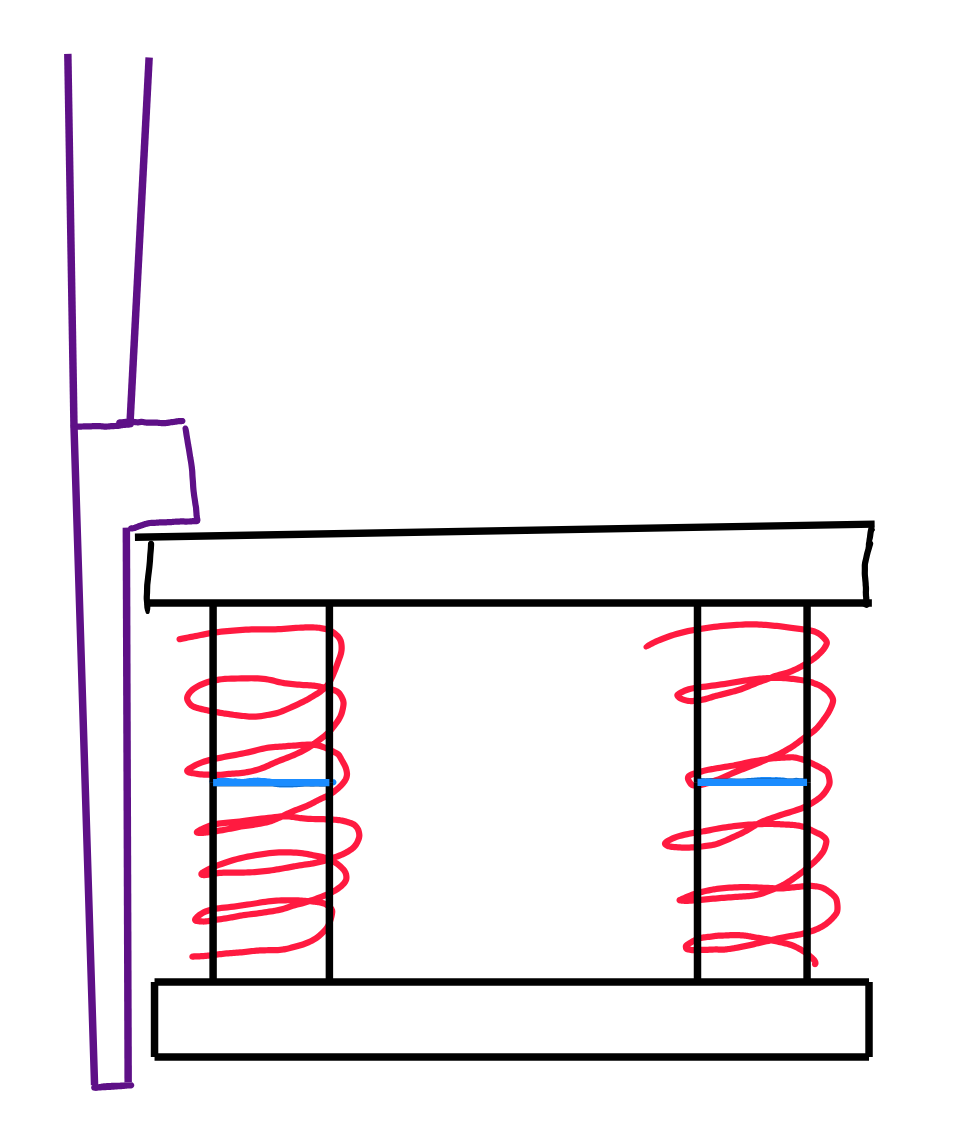
\includegraphics[width = 0.3\textwidth]{picture.png}
    \label{fig:step}
    \caption{Side view of a single step}
\end{figure}

Probably the most important
adjustment was minimising the activation energy. The final prototype is able to
be activated by the ball falling 3.5 cm. Thus, the activation energy can be
determined using the following formula.

\begin{equation}
    E_{activation} = mgh
\end{equation}

Where:
\begin{itemize}
    \item $m ~-$ Mass of golf ball
    \item $h ~-$ Height of drop
    \item $g ~-$ Gravitational constant
\end{itemize}

Using measured values, the following calculation can be made:

\[ E_{activation} = 45.2\unit{g} \cdot 9.81\unit{N\cdot  kg\inv} \cdot 3.5\unit{cm} =
15.52\unit{mJ}\]

Another observation is that once the step gets activated, friction does not
affect the mechanism in a measurable way. Additionally, the platform and the
ball remain attached until after they detach from the springs. Furthermore, the
horizontal speed remains constant, which will be used to guide the ball to
subsequent spring-step units. 

Therefore, only the vertical energy is of
interest, as it is what ensures flawless transitioning between steps. This will
be determined using the principle of conservation of energy:
\begin{gather}
    4\cdot 
    \left(\frac{k}{2}\Delta l ^{~2} \right) = (m_b + m_p)gh \\
    h = \frac{2k \Delta l^{~2}}{(m_b+m_p) g}  
\end{gather}
Where:
\begin{itemize}
    \item $\Delta l ~ -$ Spring elongation
    \item $m_b ~ -$ Mass of ball
    \item $m_p~ -$ Mass of platform
    \item $k~-$ Spring constant
\end{itemize}
Therefore, when plugging in the measurements, the following calculation ensues:
\[h = \frac{2 \cdot 4.873\unit{N\cdot m\inv} \cdot (3.1\unit{cm})^2}{(20\unit{g} +
45.2\unit{g})\cdot 9.81\unit{N\cdot kg\inv}} = 14.64\unit{cm}\]

The final observation of note is that since further compression is limited by
the spring guides, the height launch does not significantly increase with
subsequent steps.

Therefore, a simple trajectory is established, as shown in
Figure 2:

\begin{figure}[!ht]
    \centering
    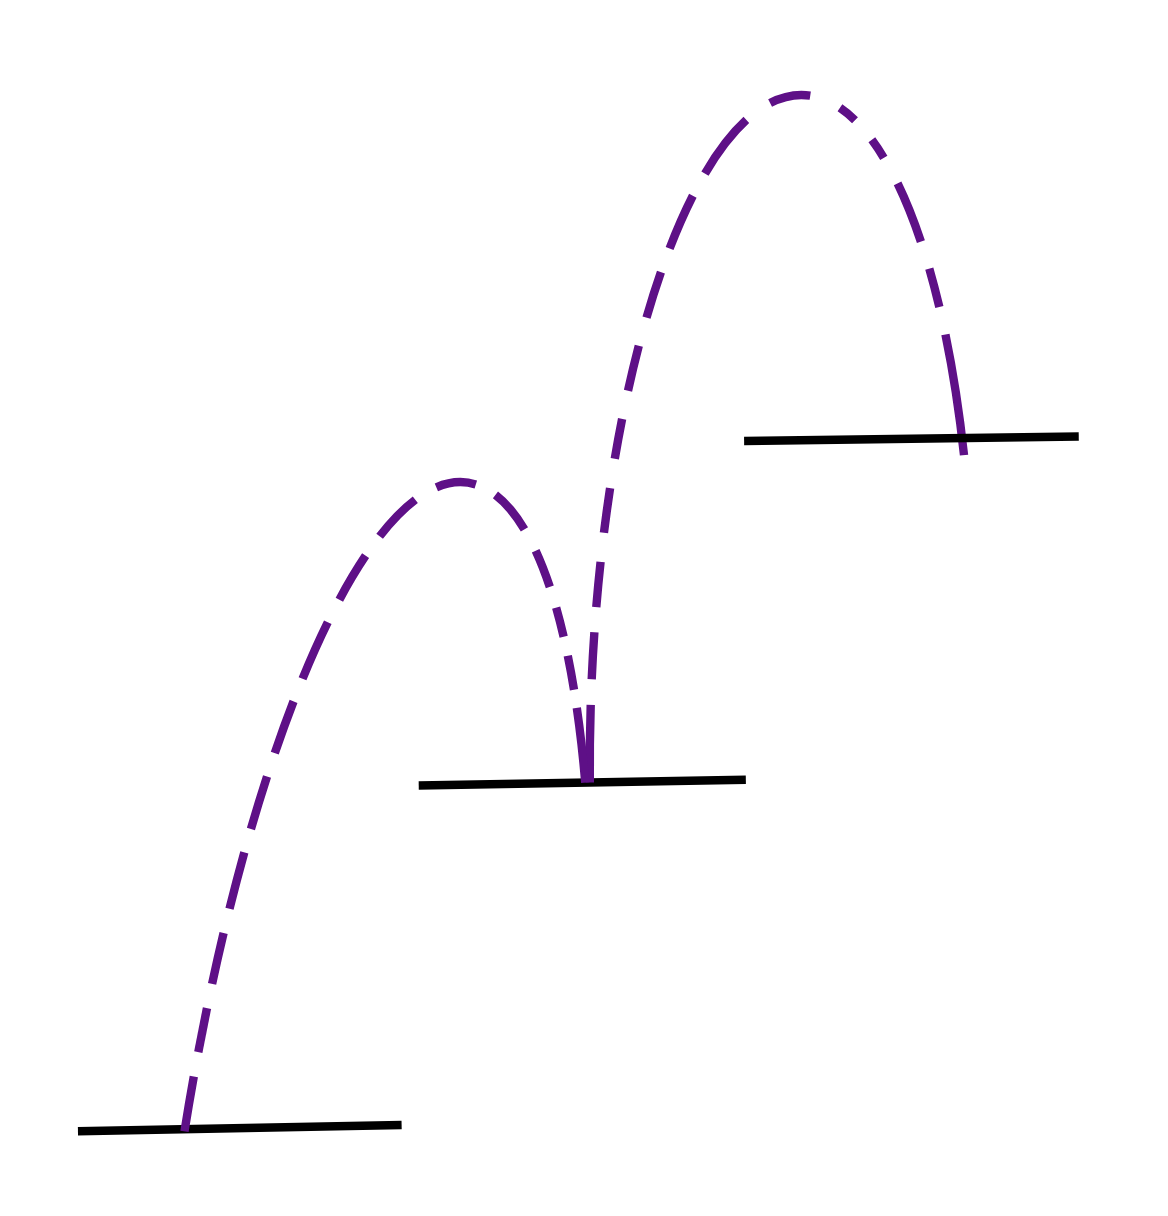
\includegraphics[width=0.3\textwidth]{trajectory.png}
    \label{fig:2}
    \caption{Visual representation of the path the ball follow}
\end{figure}

This trajectory is used to elevate the ball to the connection point between the
zones. Currently, 4 steps are needed for this transfer to be achieved.

\section{Spiral and guides}
For both the spiral and the guides, no calculations have been made, as the
movement through them is clearly slow enough, many small adjustments were made
to ensure the proper path for the ball, which makes it very difficult to
determine a regular shape for the path.

\section{Conclusion}
The calculations shown in this document have been done on the final prototype of
the Proof-of-Concept phase. As adjustments still remain to be made, these will
not be the final results of the calculations, however the results show
feasibility in our spring-step mechanism.

\section{Bibliography}
\bibliographystyle{IEEEtran}
\bibliography{Project1.bib}
\end{document}